In der Bildverarbeitung kann ein gegebenes Signal häufig nur durch eine
unstetige Funktion dargestellt werden.
Sobolev-Funktionen, obwohl im Allgemeinen nicht unbedingt stetig\todo{Quelle
für Beispiel für unstetige Funktionen sind nicht immer
Sobolev?},
lassen die oftmals benötigten Sprünge über ein-kodimensionale Mengen nicht
zu. Die Menge der Funktionen von beschränkter Variation ist 
eine echte Obermenge des Sobolev-Raums der einmal schwach differenzierbaren 
Funktionen und hat sich als geeignet für diese und weitere Anwendungen erwiesen 
(cf. \cites[398]{ABM14}[42]{AK06}[297]{Bar15}[S. 1 f.]{Bra98}).

\todo[inline]{Genauer sein, also schon $\Omega$ und alles definieren? 
soll man die Sachen zitieren, wenn die Formulierung davor von diesen 
Werken inspiriert ist? Sollen noch Kapitel angegeben werden?}

Eine mögliche Problemstellung in der Bildverarbeitung ist die 
Rauschunterdrück\-ung, das heißt der Versuch unerwünschtes Rauschen in einem
Signal zu verringern. Das ROF-Modell ist ein Modell-Problem dafür und sucht
eine Funtion $u:\Omega\to\Rbb$ die das Funktional
\begin{align*}
  I(u)\coloneqq |u|_{\BV(\Omega)}+\frac{\alpha}{2}\Vert
  u-g\Vert_{L^2(\Omega)}^2
\end{align*}
minimiert,
wobei $g\in L^2(\Omega)$ das gegebene verrauschte Bild beschreibt und 
$\alpha\in \Rbb_+$ ein Parameter ist, mit dem gewichtet werden kann, wie 
stark Oszillationen minimiert werden sollen, beschrieben durch den Term
$|u|_{\BV(\Omega)}$ (der aber Unstetigkeiten zulässt) und wie nahe die Lösung
$u$ an der Eingabe $g$ liegen soll, beschrieben durch den Term $\Vert
u-g\Vert_{L^2(\Omega)}^2$. (tradeoff between regularization and data fitting)

Die Wahl von einem zu kleinen $\alpha$ führt zu einer zu glatten, verwaschen
aussehenden Lösung, zu sehen zum Beispiel in den Abbildungen
\ref{fig:snr10alpha100} und \ref{fig:snr10alpha1000}, während die Wahl von
einem zu großen $\alpha$ das Rauschen kaum verringert, zu sehen zum Beispiel in
den Abbildungen \ref{fig:snr10alpha5000} und \ref{fig:snr10alpha10000}.
Für weitere Details und Referenzen zur Rauschunterdrückung und auch zu 
Möglichkeiten $\alpha$ gegebenfalls zu bestimmen, siehe \cite{Get12}.

Benannt ist das ROF-Modell nach Rudin, Osher und Fatemi, die dieses 
Problem 1992 in \cite{ROF92} vorschlugen 
(cf. \cites[1217]{Bar15a}[132]{CP10}[S. 74 f.]{Get12}).
\todo[inline]{ Vielleicht auch den Press Release zum Schwarzen Loch Bild
erwähnen oder ist das zu random?}

In \cite{Bar15}  das ROF MOdell mit Courant Elementen \todo{zitiere Courant 
Methode}
approximiert und den Algorithmus basierend auf (Quelle) anwendet.
Wir betrachten folgende leicht andere Formuliereung des ROF Modell 
(Problem)
und nutzen die CR FEM um die Lösung des nichtkonformen Problem
(Problem) zu bestimmen.

\begin{remark}
  In \cite[Kapitel~10.1.3]{Bar15} wird \Cref{prob:continuousProblem} für ein
  gegebenes $g\in L^2(\Omega)$ formuliert
  mit dem Funktional 
  \begin{align*}
    I(v)\coloneqq |v|_{\BV(\Omega)} + \frac{\alpha}{2}\int_\Omega (v-g)^2\dx
  \end{align*}
  für $v\in \BV(\Omega)\cap L^2(\Omega)$.

  Nun wählen wir $f = \alpha g$. Dann gilt
  $I(v) = E(v) - \Vert v\Vert_{L^1(\partial \Omega)}+ 
  \frac{\alpha}{2}\Vert g\Vert_{L^2(\Omega)}^2$ für alle 
  $v\in \BV(\Omega)\cap L^2(\Omega)$. Da der Term $\frac{\alpha}{2}\Vert
  g\Vert_{L^2(\Omega)}^2$ konstant ist, haben die Funktionale $E$ und $I$ somit
  die gleichen Minimierer in $\left\{v\in\BV(\Omega)\cap L^2(\Omega)\mid 
  \Vert v\Vert_{L^1(\partial\Omega)}=0\right\}$.
\end{remark}

In dieser Arbeit werden in Kapitel 2 (todo refs machen für Kapitel und nutzen)
zunächst die benötigten theoretischen Grundlangen zur Variationsrechnung und
Optimierung in Banachräumen als auch die relevanten Eigenschaften des
Raumes der Funktionen von beschränkter Variation (ggf. ergänzen, falls noch
mehr passiert irgendwann.

In Kapitel 3 folgt die Formulierung des konitnuierlichen Problems und des
Existenz- und Eindeutigkeitsbeweis für Minimiert des Problems. Außerdem 
wird die starke Konverxität des Energiefunktinals gezeigt für die später
numerische Auswerung.

Die Diskretisierung der nichtkonformen (sic?) Formulierung  des Problems 
und der Beweis der Existenz und Eindeutigkeit von Minimierern des 
diskreten Problems geschieht anschließend in Kapitel 4.

Kapitel 5 beschreibt den Algorithmus und beweist Konvergenz der 
Iterate. 

Kapitel 6 Implementierung und erklärt, wie das Programm genutzt werden kann.
Insbesondere wird auch erläutert, wie die Ergebnisse, die in 
\Cref{fig:exampleDenoising} zu sehen sind, reproduziert werden können.

Kapitel 7 nutzt das Programm für Experimente, die dort ausgewertet werden.

\begin{figure}[h]
  \centering
  \begin{subfigure}[b]{.4\linewidth}
    \caption{\url{https://homepages.cae.wisc.edu/~ece533/images/cameraman.tif}}
    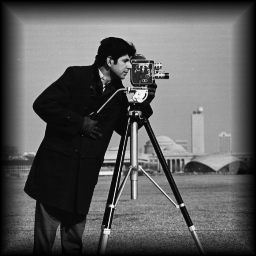
\includegraphics[width=\linewidth]{pictures/introBeta/cameraman.png}
    \label{fig:camerman}
  \end{subfigure}
  \quad
  \begin{subfigure}[b]{.4\linewidth}
    \caption{$\snr=10$}
    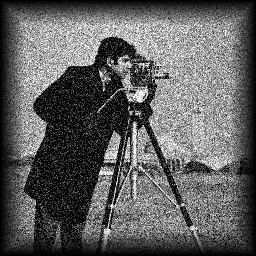
\includegraphics[width=\linewidth]{pictures/introBeta/snr10.png}
    \label{fig:camermanSNR10}
  \end{subfigure}

  \begin{subfigure}{.3\linewidth}
    \caption{$\alpha=100$}
    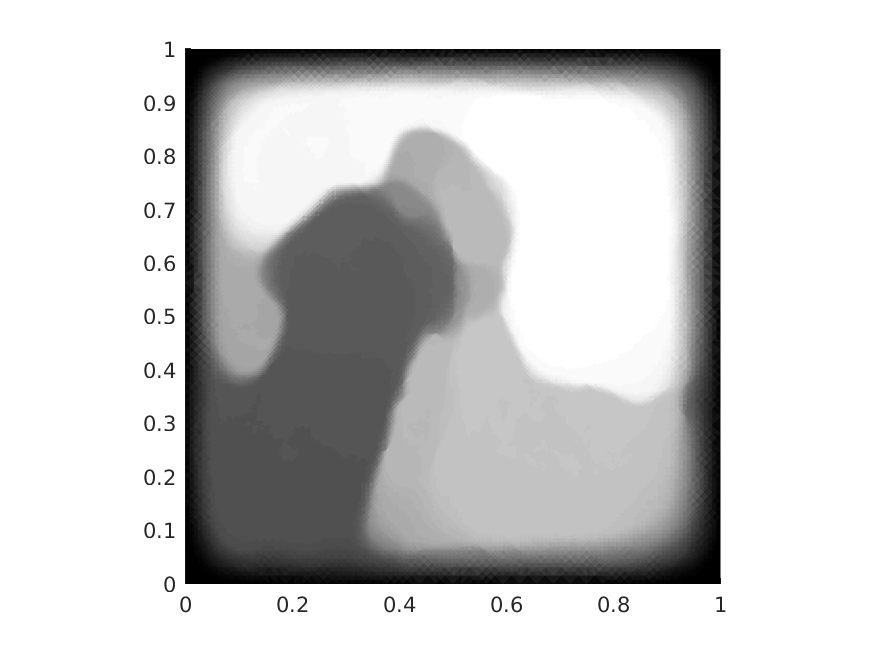
\includegraphics[trim = 60 0 60 20, clip, width=\linewidth]
      {pictures/introBeta/snr10/00100.png}
    \label{fig:snr10alpha100}
  \end{subfigure}
  \begin{subfigure}{.3\linewidth}
    \caption{$\alpha=1000$}
    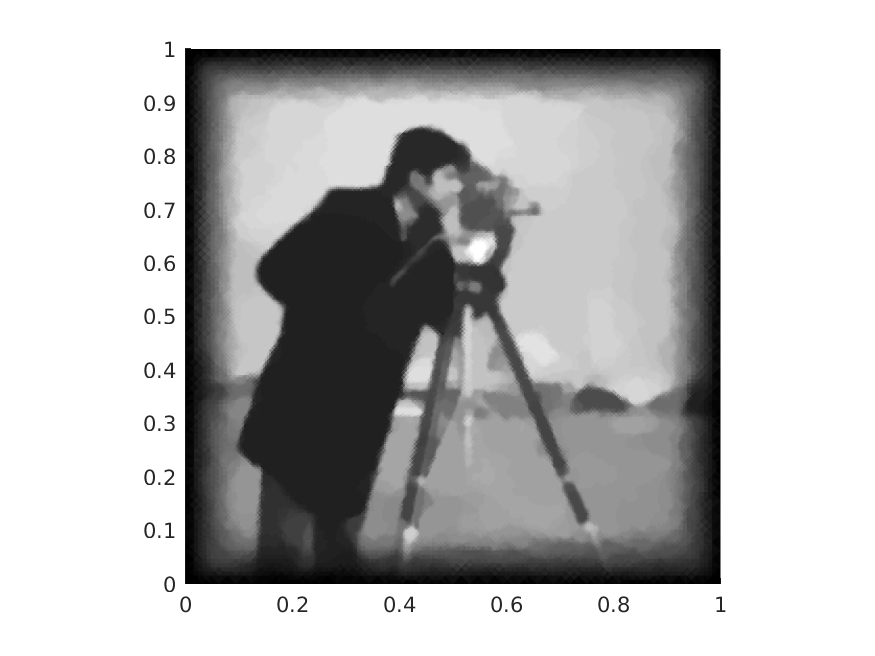
\includegraphics[trim = 60 0 60 20, clip, width=\linewidth]
      {pictures/introBeta/snr10/01000.png}
    \label{fig:snr10alpha1000}
  \end{subfigure}
  \begin{subfigure}{.3\linewidth}
    \caption{$\alpha=2500$}
    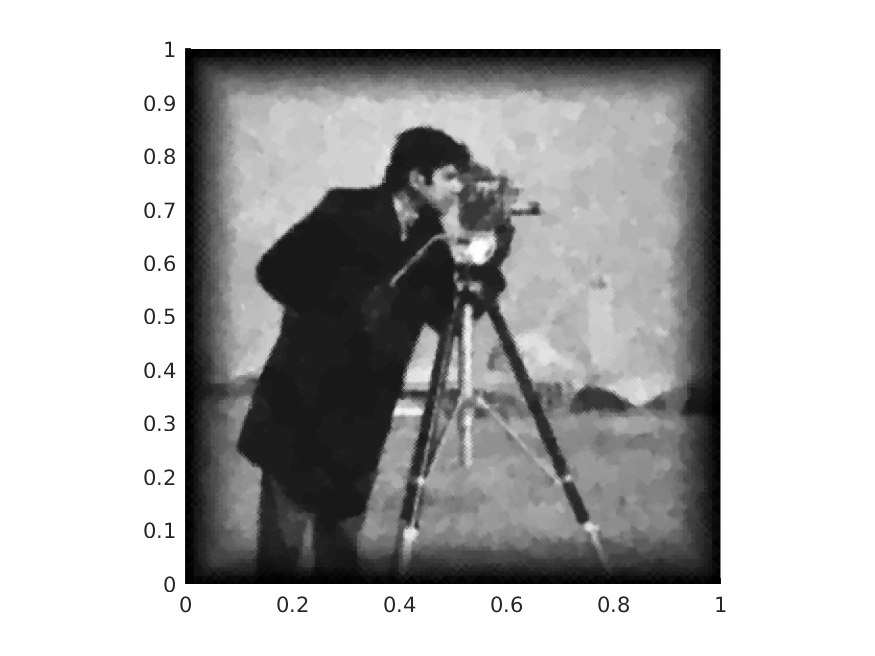
\includegraphics[trim = 60 0 60 20, clip, width=\linewidth]
      {pictures/introBeta/snr10/02500.png}
    \label{fig:snr10alpha2500}
  \end{subfigure}

  \begin{subfigure}{.3\linewidth}
    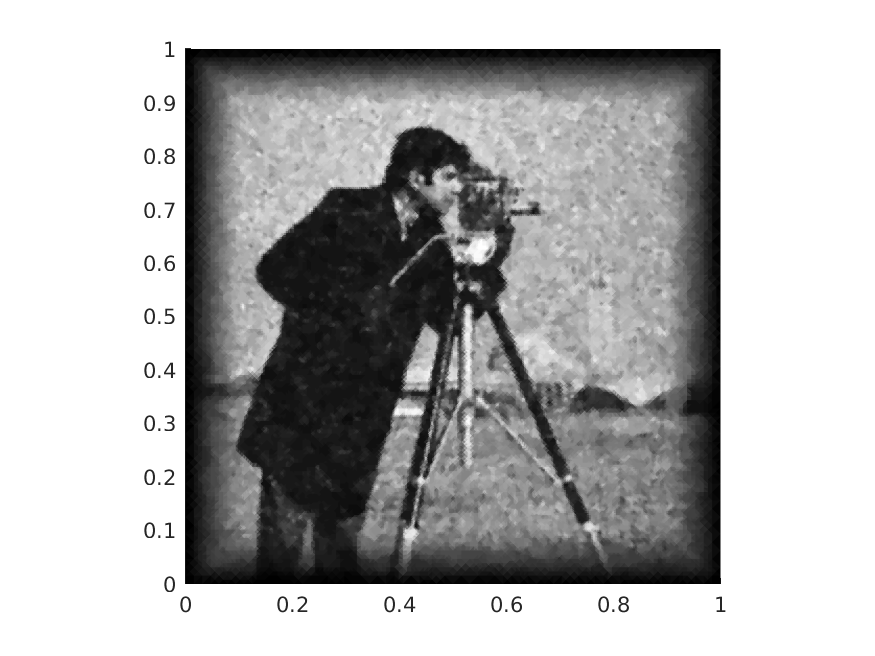
\includegraphics[trim = 60 0 60 20, clip, width=\linewidth]
      {pictures/introBeta/snr10/05000.png}
    \caption{$\alpha=05000$}
    \label{fig:snr10alpha5000}
  \end{subfigure}
  \begin{subfigure}{.3\linewidth}
    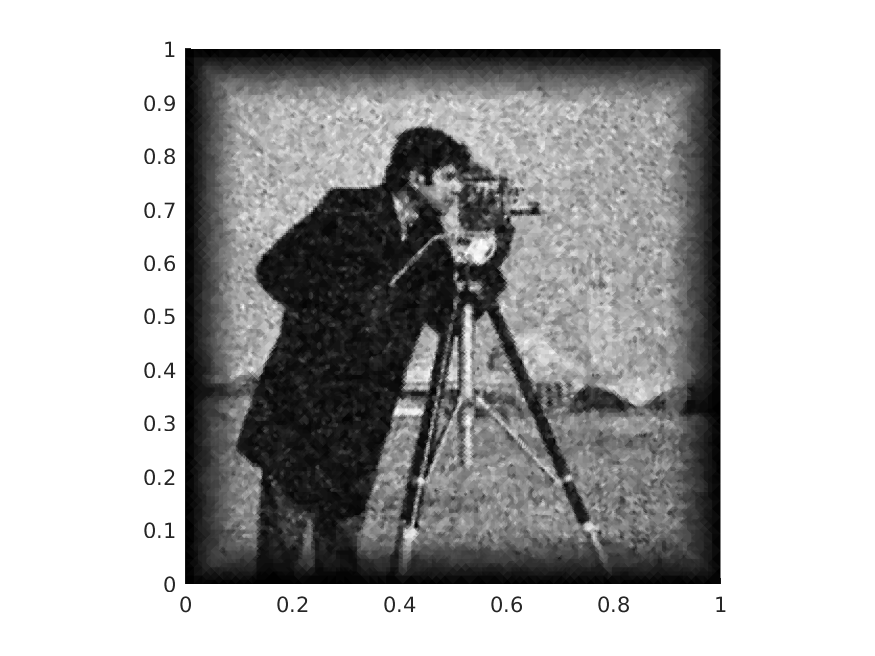
\includegraphics[trim = 60 0 60 20, clip, width=\linewidth]
      {pictures/introBeta/snr10/10000.png}
    \caption{$\alpha=10000$}
    \label{fig:snr10alpha10000}
  \end{subfigure}
  \caption{Originalbild (a) und Originalbild mit additiven weißen gaußschen
  Rauschen (b) mit einem Signal-Rausch-Verhältnis (eng.\ signal-to-noise
  ratio, SNR) von 10, jeweils mit nachträglich hinzugefügten graduellen
  Übergang zu schwarzen Rand, was Nullranddaten entspricht und drei Ergebnisse
  (c)-(g) des adaptiven Algorithmus mit verschiedenen Werten von $\alpha$}
  \label{fig:exampleDenoising}
\end{figure}

\todo[inline]{Experimente länger rechnen und vielleicht 9 Wahlen für alpha mit
einem ernsthaften Versuch, ein gut aussehendes entrauschtes Bild zu bekommen}

\begin{figure}
  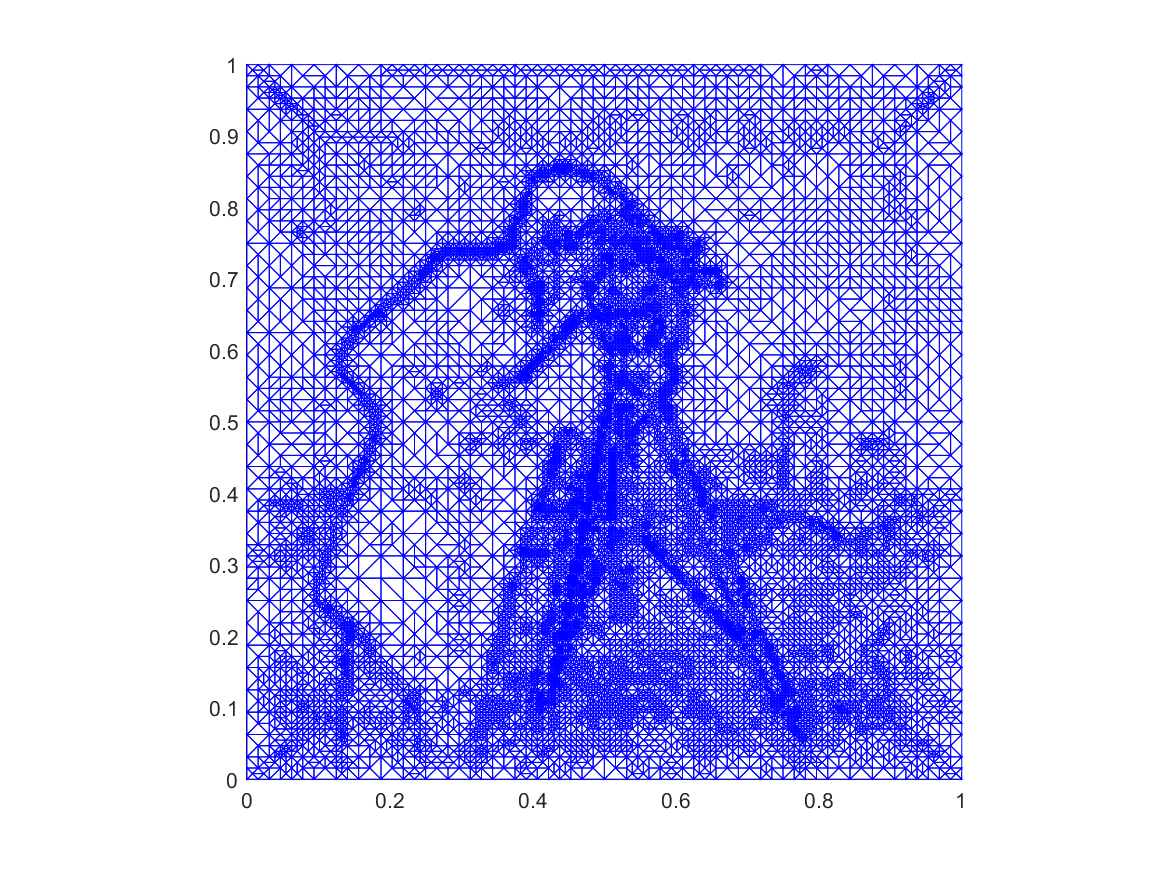
\includegraphics[trim = 60 0 60 0, clip, width=\linewidth]
    {pictures/introBeta/triangulation/triangulation.png}
  \label{fig:exampleTriangulation}
  \caption{Triangulierung mit 40300 Freiheitsgraden erzeugt vom adaptiven
  Algorithmus für rauschfreien Input}
\end{figure}

\todo[inline]{diese Triangulierungs Figure lieber in den Experimente und hier
(und zwar ausschließlich hier) die verrauschungsbeispiele bringen}
